\documentclass[aspectratio=169,11pt]{beamer}

\usetheme{Madrid}
\usecolortheme{seahorse}
\usefonttheme{professionalfonts}

\usepackage{amsmath,amssymb}
\usepackage{graphicx}
\usepackage{booktabs}
\usepackage{array}
\usepackage{xcolor}
\usepackage{tikz}
\usepackage{microtype}

\graphicspath{{../reports/}}

% ── colour palette ─────────────────────────────────────────────────────────
\definecolor{primary}{RGB}{31,73,125}     % dark blue
\definecolor{accent}{RGB}{192,0,0}        % red
\definecolor{good}{RGB}{0,128,0}          % green
\definecolor{mid}{RGB}{255,140,0}         % orange

\setbeamercolor{frametitle}{bg=primary,fg=white}
\setbeamercolor{title}{fg=white}
\setbeamercolor{subtitle}{fg=white!80}
\setbeamercolor{author}{fg=white}
\setbeamercolor{date}{fg=white!70}
\setbeamercolor{structure}{fg=primary}

% ── helpers ────────────────────────────────────────────────────────────────
\newcommand{\hi}[1]{\textcolor{accent}{\textbf{#1}}}
\newcommand{\ok}[1]{\textcolor{good}{\textbf{#1}}}
\newcommand{\warn}[1]{\textcolor{mid}{\textbf{#1}}}

\setbeamertemplate{navigation symbols}{}
\setbeamertemplate{footline}[frame number]

% ───────────────────────────────────────────────────────────────────────────
\title[Elliptic Anomaly Detection]{Graph-Aware Anomaly Detection\\
       for Blockchain Forensics}
\subtitle{A 48-Experiment Benchmark on the Elliptic Bitcoin Dataset}
\author{Sajjad Shahali Ramsheh}
\institute{Department of Control \& Computer Engineering (DAUIN)\\
           Politecnico di Torino}
\date{June 2026}

% ───────────────────────────────────────────────────────────────────────────
\begin{document}

% ── SLIDE 1: Title ──────────────────────────────────────────────────────────
\begin{frame}
  \titlepage
\end{frame}

% ── SLIDE 2: Outline ────────────────────────────────────────────────────────
\begin{frame}{Outline}
  \tableofcontents[hidesubsections]
\end{frame}

\section{Problem \& Dataset}

% ── SLIDE 3: Problem ────────────────────────────────────────────────────────
\begin{frame}{Why Bitcoin Forensics is Hard}
  \begin{columns}[T]
    \begin{column}{0.48\textwidth}
      \textbf{The setting}\\[4pt]
      \begin{itemize}
        \item Bitcoin blockchain: fully \textbf{public} but \textbf{pseudonymous}
        \item Every transaction recorded; wallet identity is hidden
        \item Money laundering, ransomware, darknet markets
        \item Traditional AML requires verified identity --- unavailable here
      \end{itemize}
    \end{column}
    \begin{column}{0.48\textwidth}
      \textbf{Three core challenges}\\[4pt]
      \begin{enumerate}
        \item \hi{Severe imbalance} --- only \hi{2\%} illicit\\
              Accuracy is useless (93.5\% by predicting all-licit)
        \item \hi{Concept drift} --- illicit rate drops\\
              11.6\% $\to$ 6.5\% train$\to$test
        \item \hi{Anonymous features} --- 165 features,\\
              semantics unpublished
      \end{enumerate}
    \end{column}
  \end{columns}
  \vfill
  \centering
  \colorbox{primary!10}{\parbox{0.9\textwidth}{\centering
    \textbf{Primary metric:} F1 on illicit class \quad
    \textbf{Secondary:} PR-AUC, ROC-AUC\\
    \small Accuracy deliberately excluded --- misleading under 6.5\% positive rate
  }}
\end{frame}

% ── SLIDE 4: Dataset ────────────────────────────────────────────────────────
\begin{frame}{The Elliptic Dataset}
  \begin{columns}[T]
    \begin{column}{0.42\textwidth}
      \begin{tabular}{@{}lr@{}}
        \toprule
        \textbf{Property} & \textbf{Value} \\
        \midrule
        Transactions       & 203\,769 \\
        Directed edges     & 234\,355 \\
        Avg.\ node degree  & 2.30 \\
        \midrule
        Illicit (label 1)  & 4\,545 (2\%) \\
        Licit (label 2)    & 42\,019 (21\%) \\
        Unlabeled          & 157\,205 (77\%) \\
        \midrule
        Time steps         & 49 \\
        Local features     & 93 \\
        Aggregated feat.   & 71 \\
        \bottomrule
      \end{tabular}
    \end{column}
    \begin{column}{0.55\textwidth}
      \textbf{Temporal split (mandatory)}\\[4pt]
      \begin{itemize}
        \item \ok{Train}: steps 1--34 \quad 29\,894 labeled rows \quad 11.6\% illicit
        \item \warn{Val}: steps 30--34 \quad (subset of train)
        \item \hi{Test}: steps 35--49 \quad 16\,670 labeled rows \quad 6.5\% illicit
      \end{itemize}
      \vspace{6pt}
      \colorbox{accent!10}{\parbox{\linewidth}{
        \small Random shuffling \textbf{leaks the future} into training
        and inflates every metric. All 48 experiments respect
        the causal time ordering.
      }}
    \end{column}
  \end{columns}
\end{frame}

% ── SLIDE 5: Concept Drift ──────────────────────────────────────────────────
\begin{frame}{Concept Drift: Illicit Rate Per Time Step}
  \begin{center}
    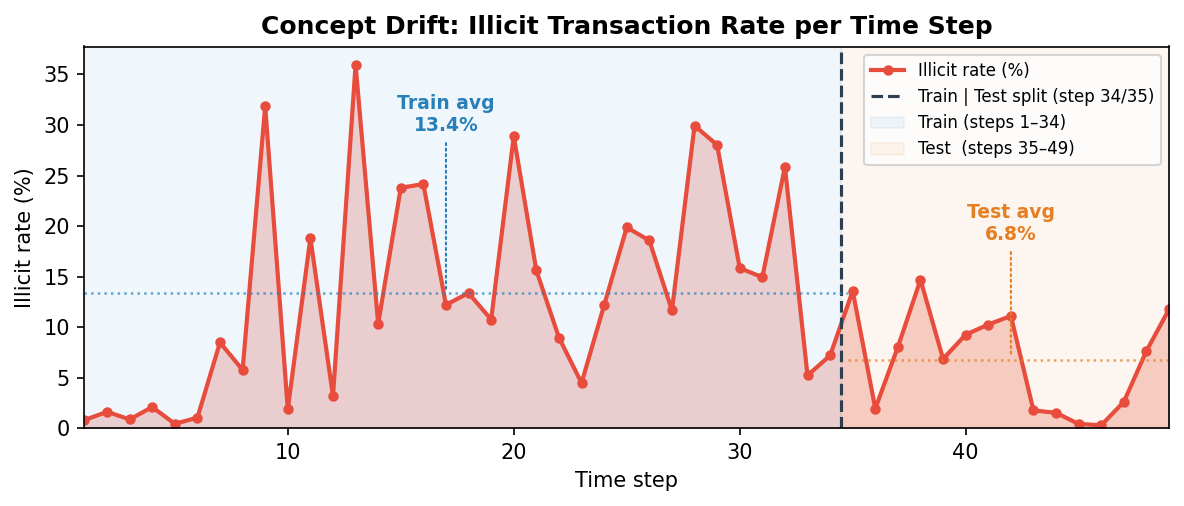
\includegraphics[width=0.88\textwidth]{concept_drift.png}
  \end{center}
  \vspace{-4pt}
  \small
  Illicit rate falls \hi{44\% relatively} from train to test window.
  Not noise --- genuine behavioural shift requiring temporal-aware evaluation.
\end{frame}

\section{Methodology}

% ── SLIDE 6: 5 Paradigms ────────────────────────────────────────────────────
\begin{frame}{Five Experimental Paradigms --- 48 Variants, 5 Rounds}
  \begin{columns}[T]
    \begin{column}{0.48\textwidth}
      \begin{enumerate}
        \item \textbf{Classical Unsupervised}\\
              IsoForest, LOF, OCSVM, spectral\\
              \textit{Train on all / licit-only rows; no labels}
        \item \textbf{Supervised Trees}\\
              LR, RF, GBM, LightGBM, Optuna-tuned\\
              \textit{Train on 29\,894 labeled rows}
        \item \textbf{Neural Anomaly Detection}\\
              AE, DenoisingAE, VAE, $\beta$-VAE, LSTM-AE\\
              \textit{Train on 26\,432 licit-only rows}
      \end{enumerate}
    \end{column}
    \begin{column}{0.48\textwidth}
      \begin{enumerate}
        \setcounter{enumi}{3}
        \item \textbf{GNN Supervised}\\
              GraphSAGE family, GAT, GATv2\\
              \textit{Full graph, node-mask training}
        \item \textbf{Semi-supervised / Ensemble}\\
              Pseudo-labels, weighted ensemble,\\
              Platt / isotonic calibration
      \end{enumerate}
      \vspace{8pt}
      \colorbox{primary!10}{\parbox{\linewidth}{
        \small \textbf{Course-derived methods:}\\
        DOMINANT, LSTM-AE, $\beta$-VAE, EVT\\
        thresholding, spectral embedding,\\
        pseudo-label propagation
      }}
    \end{column}
  \end{columns}
\end{frame}

\section{Results}

% ── SLIDE 7: 5 Tiers Overview ───────────────────────────────────────────────
\begin{frame}{Five Performance Tiers Across 48 Experiments}
  \begin{columns}[T]
    \begin{column}{0.50\textwidth}
      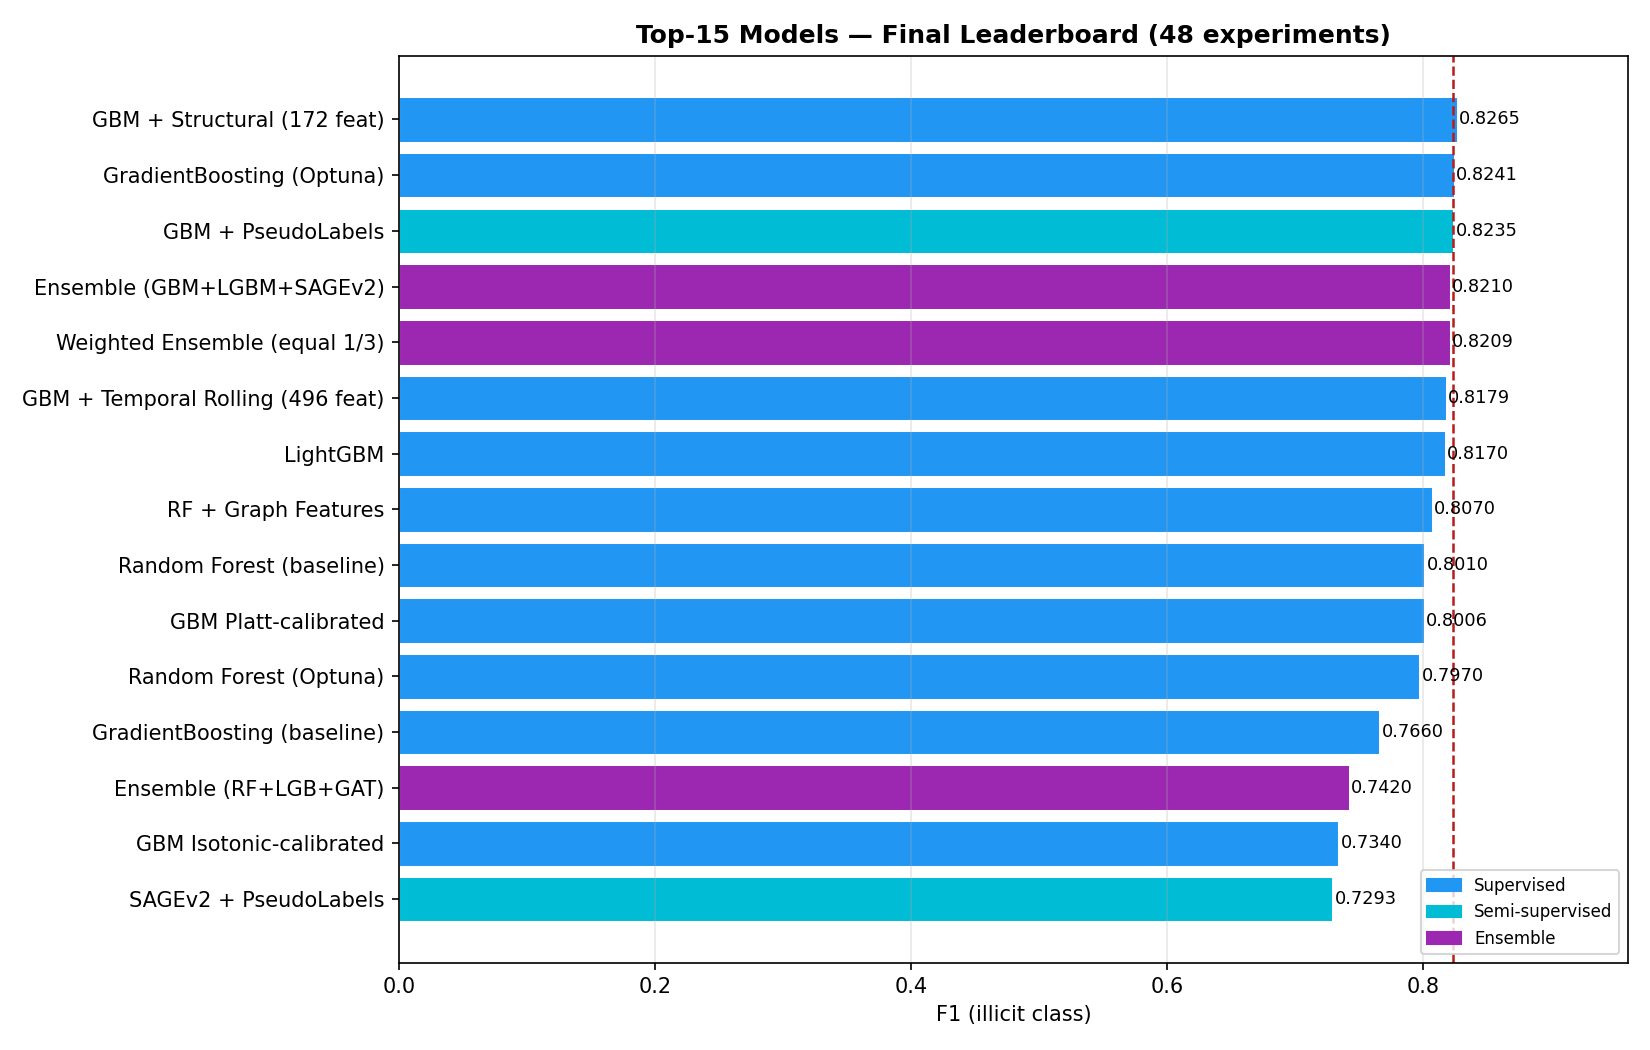
\includegraphics[width=\textwidth]{final_top15_f1.png}
    \end{column}
    \begin{column}{0.47\textwidth}
      \vspace{4pt}
      \begin{tabular}{@{}lc@{}}
        \toprule
        \textbf{Tier} & \textbf{F1 range} \\
        \midrule
        \ok{Supervised / Ensemble}  & 0.74--\ok{0.83} \\
        \ok{GNN supervised}         & 0.54--0.73 \\
        \warn{Neural AE}            & 0.12--0.41 \\
        \warn{Graph AE (DOMINANT)}  & 0.21 \\
        \hi{Classical unsupervised} & $<$0.10 \\
        \bottomrule
      \end{tabular}
      \vspace{10pt}
      \begin{block}{Key insight}
        \small Supervised trees dominate because the 71 aggregated
        features already encode neighbourhood signal in tabular form.
        GBM + structural topology: \ok{F1 = 0.8265}
      \end{block}
    \end{column}
  \end{columns}
\end{frame}

% ── SLIDE 8: Supervised + Round Progression ─────────────────────────────────
\begin{frame}{Supervised Results \& Improvement Journey}
  \begin{columns}[T]
    \begin{column}{0.52\textwidth}
      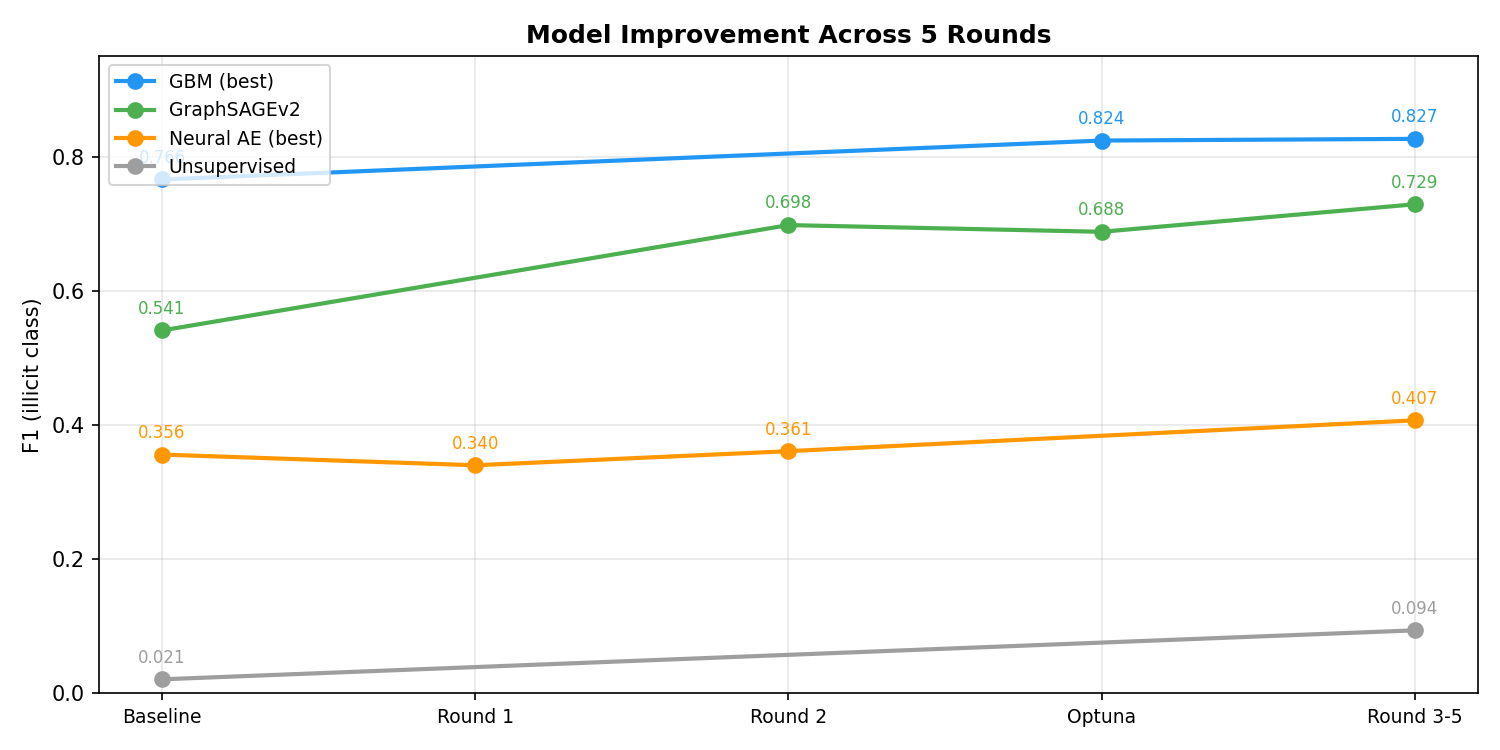
\includegraphics[width=\textwidth]{final_round_progression.png}
    \end{column}
    \begin{column}{0.45\textwidth}
      \vspace{4pt}
      \textbf{Best supervised results:}\\[4pt]
      \begin{tabular}{@{}lc@{}}
        \toprule
        Model & F1 \\
        \midrule
        GBM + Structural & \ok{0.827} \\
        GBM Optuna       & 0.824 \\
        LightGBM         & 0.817 \\
        Random Forest    & 0.801 \\
        Logistic Reg.    & 0.302 \\
        \bottomrule
      \end{tabular}
      \vspace{8pt}
      \small
      \begin{itemize}
        \item Optuna (+0.058 over GBM baseline)
        \item Structural topology adds +0.002 on top
        \item Semi-supervised pseudo-labels: $\Delta{=}-0.0006$ (already saturated)
      \end{itemize}
    \end{column}
  \end{columns}
\end{frame}

% ── SLIDE 9: GNN Ablation ───────────────────────────────────────────────────
\begin{frame}{GNN Ablation: What Actually Matters?}
  \begin{columns}[T]
    \begin{column}{0.52\textwidth}
      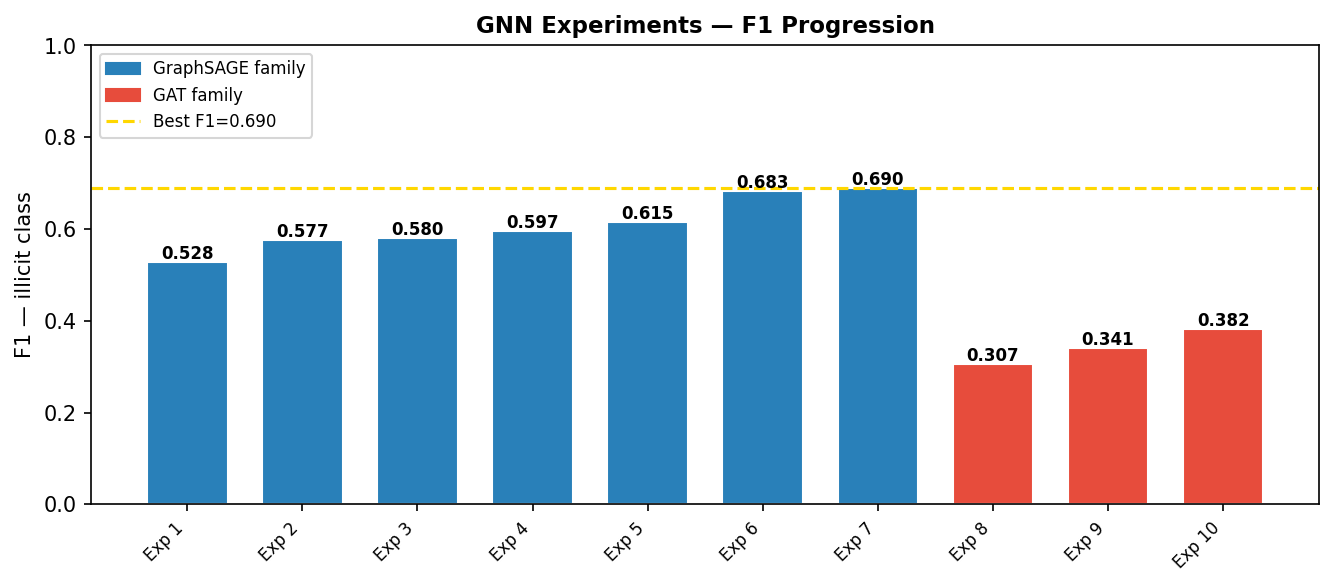
\includegraphics[width=\textwidth]{gnn_stacked_top.png}
    \end{column}
    \begin{column}{0.45\textwidth}
      \vspace{4pt}
      \textbf{10 controlled experiments:}\\[6pt]
      \begin{tabular}{@{}lc@{}}
        \toprule
        Design choice & $\Delta$F1 \\
        \midrule
        \ok{LayerNorm + self-loops} & \ok{+0.068} \\
        Depth (2L $\to$ 3L)        & +0.038 \\
        Width (h=64 $\to$ 256)     & +0.052 \\
        Optuna lr tuning            & +0.007 \\
        \midrule
        \hi{GAT / GATv2}           & \hi{$-$0.308 vs SAGE} \\
        \bottomrule
      \end{tabular}
      \vspace{8pt}
      \begin{alertblock}{Finding}
        \small Attention is noisy on sparse graphs (avg.\ degree 2.3).
        Mean aggregation (GraphSAGE) wins.\\
        Best GNN: GraphSAGEv2 \ok{F1 = 0.698}\\
        = \ok{84.5\%} of supervised ceiling
      \end{alertblock}
    \end{column}
  \end{columns}
\end{frame}

% ── SLIDE 10: Unsupervised + Neural AE ──────────────────────────────────────
\begin{frame}{Unsupervised Detection: Score Inversion Paradox}
  \begin{columns}[T]
    \begin{column}{0.50\textwidth}
      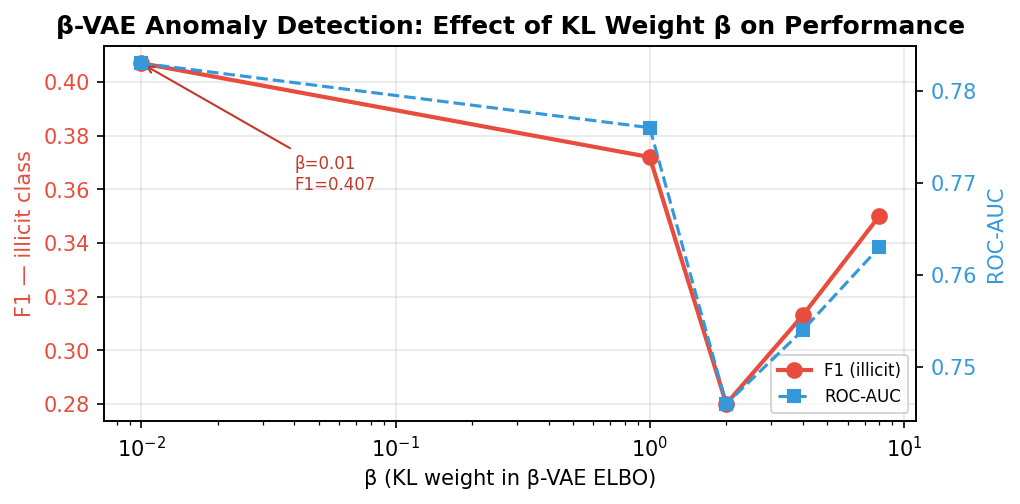
\includegraphics[width=\textwidth]{beta_f1_curve.png}
    \end{column}
    \begin{column}{0.47\textwidth}
      \vspace{4pt}
      \textbf{Classical unsupervised: all fail}\\
      IsoForest F1=0.021, LOF F1=0.076\\[6pt]
      \colorbox{accent!10}{\parbox{\linewidth}{
        \small \textbf{Score inversion:} illicit transactions
        reconstruct with \textit{lower} MSE than licit ones.
        Anomaly score must be $-$MSE, not $+$MSE.\\
        Laundering patterns are \textbf{stereotyped}, not rare.
      }}
      \vspace{6pt}
      \textbf{Best unsupervised results:}\\[4pt]
      \begin{tabular}{@{}lc@{}}
        \toprule
        Model & F1 \\
        \midrule
        $\beta$-VAE ($\beta{=}0.01$) & \ok{0.407} \\
        DenoisingAE                  & 0.361 \\
        DOMINANT (graph AE)          & 0.212 \\
        Classical best (LOF)         & 0.076 \\
        \bottomrule
      \end{tabular}
    \end{column}
  \end{columns}
\end{frame}

% ── SLIDE 11: PR Curves ─────────────────────────────────────────────────────
\begin{frame}{Precision--Recall Curves: Supervised Models}
  \begin{columns}[T]
    \begin{column}{0.55\textwidth}
      
\includegraphics[width=\textwidth]{pr_curves.png}
    \end{column}
    \begin{column}{0.42\textwidth}
      \vspace{10pt}
      \begin{tabular}{@{}lc@{}}
        \toprule
        Model & AP \\
        \midrule
        LightGBM       & \ok{0.806} \\
        GBM Optuna     & 0.804 \\
        GBM baseline   & 0.800 \\
        Random Forest  & 0.797 \\
        Logistic Reg.  & 0.291 \\
        Chance line    & 0.065 \\
        \bottomrule
      \end{tabular}
      \vspace{10pt}
      \small
      PR-AUC is \textbf{threshold-independent} and informative
      under imbalance --- it ignores the large pool of true
      negatives that inflates ROC-AUC.
    \end{column}
  \end{columns}
\end{frame}

\section{Explainability}

% ── SLIDE 12: SHAP ──────────────────────────────────────────────────────────
\begin{frame}{Cross-Paradigm Feature Agreement}
  \begin{columns}[T]
    \begin{column}{0.52\textwidth}
      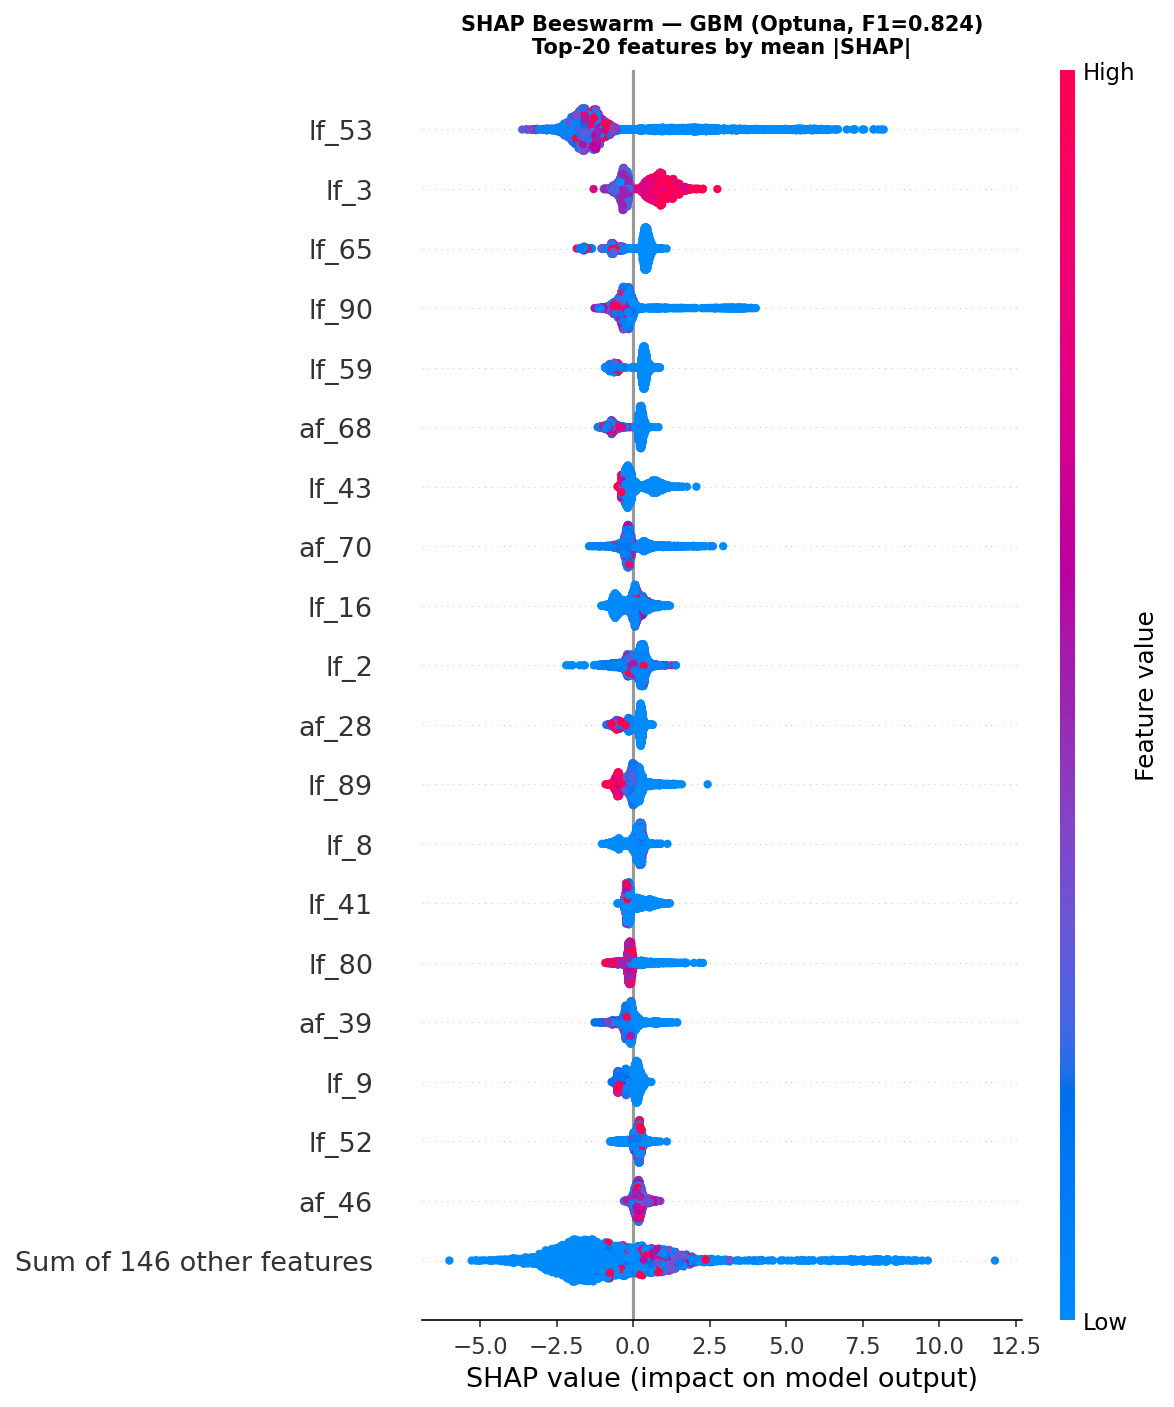
\includegraphics[width=\textwidth]{shap_gbm_beeswarm.png}
    \end{column}
    \begin{column}{0.45\textwidth}
      \vspace{4pt}
      \textbf{Method:}\\
      \begin{itemize}
        \item SHAP TreeExplainer $\to$ GBM
        \item Gradient attribution $\to$ GraphSAGE
      \end{itemize}
      \vspace{6pt}
      \textbf{Cross-paradigm consensus (top-20 in all models):}\\[4pt]
      \begin{center}
      \colorbox{good!20}{\texttt{lf\_53}} \quad
      \colorbox{good!20}{\texttt{lf\_90}} \quad
      \colorbox{good!20}{\texttt{af\_70}}
      \end{center}
      \vspace{6pt}
      \small
      \begin{itemize}
        \item \texttt{lf\_*} = local transaction features
        \item \texttt{af\_*} = aggregated neighbourhood feature
        \item \texttt{af\_70} in GNN attribution confirms\\
              \textbf{graph signal exists} beyond tabular proxies
        \item Semantics unknown --- requires Elliptic collaboration
      \end{itemize}
    \end{column}
  \end{columns}
\end{frame}

\section{Conclusions}

% ── SLIDE 13: RQ Answers ────────────────────────────────────────────────────
\begin{frame}{Research Questions --- Answered}
  \begin{tabular}{@{}p{0.08\textwidth}p{0.87\textwidth}@{}}
    \toprule
    \textbf{RQ} & \textbf{Answer} \\
    \midrule
    \textbf{RQ1} &
      Classical unsupervised detectors \hi{fail} (F1 $<$ 0.10).
      Illicit transactions are \textbf{stereotyped, not rare} --- they form
      dense clusters, not outliers. \\[4pt]
    \textbf{RQ2} &
      GraphSAGEv2 recovers \ok{84.5\%} of the supervised ceiling
      using only graph message passing.
      GBM and GNN exploit \textbf{complementary channels}. \\[4pt]
    \textbf{RQ3} &
      \ok{LayerNorm+self-loops} ($+$0.068) $>$ depth ($+$0.038)
      $>$ width $>$ tuning.
      \hi{Attention underperforms} mean aggregation on sparse graphs. \\[4pt]
    \textbf{RQ4} &
      \ok{\texttt{lf\_53}}, \ok{\texttt{lf\_90}}, \ok{\texttt{af\_70}}
      rank top-20 in RF, GBM, and GraphSAGE --- robust cross-paradigm signals. \\
    \bottomrule
  \end{tabular}
\end{frame}

% ── SLIDE 14: Conclusions ───────────────────────────────────────────────────
\begin{frame}{Conclusions}
  \begin{columns}[T]
    \begin{column}{0.48\textwidth}
      \textbf{6 key findings:}
      \begin{enumerate}\small
        \item \textbf{Temporal split is mandatory}\\
              Random shuffling invalidates all metrics
        \item \textbf{Supervised trees dominate}\\
              GBM + structural: \ok{F1 = 0.8265}
        \item \textbf{GNNs add complementary signal}\\
              GraphSAGEv2: \ok{F1 = 0.698} (84.5\% of ceiling)
        \item \textbf{AE detection is viable but inverted}\\
              $\beta$-VAE ($\beta{=}0.01$): F1 = 0.407
        \item \textbf{DOMINANT best unsupervised graph method}\\
              F1 = 0.212, beats all classical by $>$0.13
        \item \textbf{Robust cross-paradigm features exist}\\
              \texttt{lf\_53}, \texttt{lf\_90}, \texttt{af\_70}
      \end{enumerate}
    \end{column}
    \begin{column}{0.48\textwidth}
      \textbf{Future work:}
      \begin{itemize}\small
        \item GBM + GraphSAGEv2 stacking ensemble
        \item Per-transaction LSTM-AE
        \item EvolveGCN for temporal drift
        \item Online threshold recalibration
        \item GNNExplainer for node-level attribution
        \item Elliptic collaboration: feature semantics
      \end{itemize}
      \vspace{10pt}
      \begin{block}{Bottom line}
        \small On Elliptic, illicit transactions are not outliers.
        Supervised trees + graph structure together provide the
        strongest forensic signal. Course-derived unsupervised
        methods ($\beta$-VAE, DOMINANT) are viable baselines.
      \end{block}
    \end{column}
  \end{columns}
\end{frame}

% ── SLIDE 15: Thank you ─────────────────────────────────────────────────────
\begin{frame}[plain]
  \begin{center}
    \vspace{1.5cm}
    {\LARGE \textbf{Thank You}}\\[0.5cm]
    {\large Questions?}\\[1.5cm]
    \begin{tabular}{ll}
      \textbf{Student:} & Sajjad Shahali Ramsheh \\
      \textbf{Email:}   & s340464@studenti.polito.it \\
      \textbf{Course:}  & DAUIN, Politecnico di Torino \\
    \end{tabular}\\[1cm]
    \colorbox{primary!10}{\parbox{0.75\textwidth}{\centering\small
      Best result: \ok{GBM + Structural, F1 = 0.8265}\\
      Best GNN: GraphSAGEv2, F1 = 0.698\\
      Best unsupervised: $\beta$-VAE ($\beta{=}0.01$), F1 = 0.407\\
      48 experiments $\cdot$ 5 paradigms $\cdot$ strict temporal split
    }}
  \end{center}
\end{frame}

\end{document}
